

\chapter{数据的提取与处理}

要检测性能回退是否出现,我们必须要从测试的环境中获取能够对性能进行判断的相关数据,即我们要进行测试数据的提取。

\section{数据提取}

虽然在已有的研究结果\cite{Jiang:2010:AAL:1831708.1831726}中指出使用额外的监视器来获取测试数据很有可能会造成额外的消耗从而影响测试数据的可靠性,但是在我们的测试框架中,我们采用最简单的方式来实现监视器,并且使用比较低的采样频率(每秒一次)来获取测试数据,以此来降低系统监视器对测试结果造成的影响。

\subsection{系统监视器}

系统监视器,就是以某种频率从系统中读取系统状态参数的并将其记录下来的程序。在这一部分,我将详细描述我们框架中的系统监视器的设计和实现。

前面提到,在我们的测试框架中,我们将采集尽可能多的,覆盖面广的测试数据,这样,我们才进行更加细致和全面的分析,于是在我们的测试框架中,将包含表\ref{tab:monitor_type}几类的系统监视器。

\begin{table}[tbp]
\centering  % 表居中
\tablehead{\hline
	监视器类型 & 监视器功能\\
	\hline \hline}
\tabletail{\hline}

\begin{supertabular}{p{3cm}p{10cm}}
CPU类 & 用于监视和CPU相关的系统状态\\
内存类 & 主要用于监视系统中和内存管理相关得系统参数\\
I/O类 & 主要用于监视系统中得输入输出状态\\
杂类 & 监控出了CPU,内存和I/O之外得其他参数\\
\end{supertabular}
\caption{监视器分类}
\label{tab:monitor_type}
\end{table}

下面我们将分类介绍这些不同的系统监视器。
\subsubsection{CPU类系统监视器}


对于CPU类的系统监视器来说,比较重要的自然是监视系统中的CPU的负载情况和CPU负载中的不同成分(包括内核系统负载和用户态负载),在多核SMP的情况下,我们还需要分别监视每一个核的运行情况,另外,在这里,我们把进程相关的监视器也包含在CPU类系统监视器中。

表\ref{tab:cpu_monitor}中列出了在我们的框架中所使用的所有CPU类系统监视器,以及它们所能够采集的数据。

\begin{table}[tbp]
\centering  % 表居中
\tablehead{\hline
	监视器 & 监视器功能 & 相关文件\\
	\hline \hline}
\tabletail{\hline}

\begin{supertabular}{p{3cm}p{7cm}p{3cm}}
interrupts & 监视系统中每一个CPU核中各种中断发生的情况 & /proc/interrupts\\
sched\_debug & 监视系统中每一个CPU核的各种调试参数和系统信息,如时钟的频率等;此外,该监视器还监视系统中的进程运行情况,提供进程调度的相关信息 & /proc/sched\_debug\\
softirqs & 监视系统中所有CPU核上的所有软中断情况 & /proc/softirqs\\
vmstat & 使用Linux中自带的常用工具vmstat来获取当前系统中的CPU负载状态,其中将包括 & 无\\
\end{supertabular}
\caption{CPU类系统监视器}
\label{tab:cpu_monitor}
\end{table}

在操作系统中,CPU作为执行指令的工具,其功能十分复杂,中断则是CPU最重要的功能之一,了解系统的中断有助于我们了解分析系统中相关硬件和相关子系统的运行状况,在发生性能回退问题的时候能够帮助我们进行更加准确地分析和定位问题。


\subsubsection{内存类系统监视器}

内存管理是操作系统中的一个重要功能,于是内存管理子系统也成为操作系统的中最为重要的子系统之一。内存管理子系统的性能好坏也直接影响整个操作系统的性能,因此,对于一个性能测试框架来说,内存管理性能相关的参数自然是必不可少的。

在Linux内核中,内存管理子系统是相当复杂的。其中,在内存管理中,比较重要的一个内存管理算法就是buddy算法,buddy system正是使用了这个这个算法来管理内存,这个算法的性能好坏也直接影响到整个内存管理系统,因此我们使用了一些监视器来专门监视buddy算法的运行状况。

此外,Linux内核的内存管理子系统还包括了非一致内存访问(NUMA)的管理。因此,除了监视普通的内存管理系统之外,还需要对NUMA管理系统也进行监视。

为了尽可能覆盖Linux内核中内存管理子系统中的相关功能,在我们的性能测试框架中,选择了表\ref{tab:mm_monitor}中列出的系统监视器为我们提供测试数据。

\begin{table}[tbp]
\centering  % 表居中
\tablehead{\hline
	监视器 & 监视器功能 & 相关文件\\
	\hline \hline}
\tabletail{\hline}

\begin{supertabular}{p{3cm}p{7cm}p{3cm}}
buddyinfo & 监视操作系统内存管理子系统中的Buddy内存分配算法的运行状况,其中的信息既可以用来进行性能的判断计算,还可以方便内核开发者的调试和问题定位 & /proc/buddyinfo\\
meminfo & 监视操作系统中内存各方面的使用状况 & /proc/meminfo\\
slabinfo & 监视内存管理子系统中SLAB算法的运行状况,功能和buddyinfo类似,可以提供测试数据,也可方便开发者的调试 & /proc/slabinfo\\
pagetypeinfo & 和buddyinfo监视器类似,其中还收集NUMA中不同node的详细信息 & /proc/pagetypeinfo\\
zoneinfo & 在NUMA系统中收集信息,可以得到NUMA中每一个node的详细信息 & /proc/zoneinfo\\
numa-meminfo & 监视NUMA系统中每一个node的内存信息 & /sys/devices/system/node\\
numa-vmstat & 收集NUMA系统中每一个node的虚拟内存信息 & /sys/devices/system/node\\
numa-numastat & 监视NUMA中每一个node的详细运行状态 & /sys/devices/system/node\\
proc-vmstat & 提供系统中相关内存子系统的相关信息,包括内存管理和页面切换管理等 &/proc/vmstat\\
\end{supertabular}
\caption{内存类系统监视器}
\label{tab:mem_monitor}
\end{table}



\subsubsection{I/O类系统监视器}

输入输出(I/O)几乎是计算机里最为重要的一部分了,同样,对于一个操作系统来说,输入输出(I/O)子系统同样也是最为重要的一部分。

一般,I/O子系统一般包括外设的输入输出和网络操作,我们选择的系统监视器也将监视这几个方面的测试数据。

表\ref{tab:io_monitor}中列出了我们的测试框架中使用的I/O类系统监视器。

\begin{table}[tbp]
\centering  % 表居中
\tablehead{\hline
	监视器 & 监视器功能 & 相关文件\\
	\hline \hline}
\tabletail{\hline}

\begin{supertabular}{p{3cm}p{7cm}p{3cm}}
mountstats & 监视操作系统中文件系统的挂载情况,其中会给出NFS文件系统的详细运行状态,这可以对操作系统中NFS的性能进行比较详细的监视 & /proc/self/mountstats\\
nfsstat & 这是Linux系统中常用的一款NFS状态查看工具,我们将其封装成一个完整的系统监视器,可以对NFS的运行状态进行详细的汇报,有助于进行性能分析 & 无\\
iostat & 同样也是一款Linux的常用工具,其作用在于 & 无\\
\end{supertabular}
\caption{I/O类系统监视器}
\label{tab:io_monitor}
\end{table}


\subsubsection{杂类系统监视器}

除了CPU类,内存类以及I/O类三类系统监视器之外,我们还选用了一些同样非常有用的监视器,这些监视器能够帮助我们更加方便和快速地分析和定位问题,表\ref{tab:misc_monitor}列出了我们的测试框架中所使用的所有杂类系统监视器。

\begin{table}[tbp]
\centering  % 表居中
\tablehead{\hline
	监视器 & 监视器功能 & 相关文件\\
	\hline \hline}
\tabletail{\hline}

\begin{supertabular}{p{3cm}p{7cm}p{3cm}}
lock\_stat & 监视操作系统内核中各种锁的使用情况,其中包括每一个锁lock和unlock的次数,以及每一个锁的总耗时等相关信息 & /proc/lock\_stat\\
latency\_stats & 监视当前内核中函数的调用延迟信息和函数的调用栈关系 & /proc/latency\_stats\\
\end{supertabular}
\caption{杂类系统监视器}
\label{tab:misc_monitor}
\end{table}

这里我们选择了lock\_stat作为我们框架中的一个杂类系统监视器是因为在Linux操作同内核中已经实现了锁的机制,而且在内核中,锁也得到了大量的应用,在Boyd-Wickizer的论文\cite{boyd2012non}中提到,锁机制的实现对操作系统内核性能的影响非常大,特别是在多核的计算机上,锁的实现对系统内核的影响更是巨大。因此,对内核中的锁进行监视是非常有必要的,而在Linux内核中最好的监视器可以说就是lock\_stat。

在杂类系统监视器中,我们还选用了latency\_stats,latency\_stats是由Intel开发的一款Linux内核调用信息记录工具,这个监视器将会输出如下面的内容:
{
\footnotesize
\begin{verbatim}

time: 1365434000.208857599
Latency Top version : v0.1
1 1537 1537 pipe_wait pipe_read do_sync_read vfs_read sys_read system_call_fastpath
1 65 65 do_wait sys_wait4 system_call_fastpath
\end{verbatim}
}
其中第一行是一个时间戳,第二行显示的是该监视器的版本信息,第三行和第四行分别是两种调用路径发生的情况,从显示的信息来看,第三行的调用路径最终在pipe\_wait这个函数中停留了1537个单位时间才返回,第四行的调用路径最终在do\_wait这个函数停留了65个单位时间之后返回。有了这样的信息,在发生问题的时候,我们能够更加方便地定位到问题发生的位置,这对性能测试和问题分析具有重大意义。


\subsubsection{系统监视器的实现}
前面已经介绍了在我们的框架中所使用的所有系统监视器,下面来介绍每一个系统监视器的具体实现方式。

前面提到在系统监视器的实现上,我们会遵循尽可能降低系统监视器对系统造成的影响的原则,来实现系统监视器。

为了方便后期的数据处理,对于每一个系统监视器,我们都要求每一秒的输出结果都必须附带一个时间戳作为不同的时间段数据的分隔,因此,对于每一个系统监视器,输出结构都要求保持下面的格式:
\begin{verbatim}
...
...
time: A
监视器在A时刻的输出结果
time: B
监视器在B时刻的输出结果
...
...
\end{verbatim}

于是,我们的测试框架中系统监视器的实现用伪代码可以表示为:






其中$Interval$这个变量就是两次输出之间的时间间隔,由于过高的采样速率会使系统监视器产生过高的额外性能损耗,于是我们使用的采样速率为每秒一次,因此在这里,$Interval$这个变量应该设置为1秒。

除了这些需要我们实现循环输出的系统监视器之外,还有一些Linux自带的工具,如iostat和vmstat等工具,都能够通过设置命令行参数来实现定时的循环输出效果,这样的系统监视器我们直接使用自带的循环输出功能,虽然时间戳的输出格式不同,但是只要在进行输出数据处理的过程中单独处理即可。

对于我们的测试框架中大部分的系统监视器来说,输出的信息就是/proc文件夹中的某一个虚拟文件,于是,我使用使用shell脚本进行实现,以此达到简单易懂的目的。

在实现的细节上,还需要注意的是,某一些系统监视器在使用之前必须要先将Linux操作系统中的相应功能开启,如latency\_stats,在读取/proc/latency\_stats之前还需要执行下面的命令开始内核中相应的功能:

\begin{lstlisting}[language=bash]
echo 0 > /proc/latency_stats
echo 1 > /proc/sys/kernel/latencytop
\end{lstlisting}

\subsection{系统监视器数据的格式化}

在上一个部分中,已经介绍了我们的测试框架中所使用的系统监视器,在本部分,将介绍系统监视器输出数据的提取方式。

虽然在实现系统监视器的时候,我们已经要求系统监视器按照一定的格式进行输出,但是这只能保证我们能够正确地读取到正确的时间戳和相应的系统监视器输出内容,不同的系统监视器输出由于所监视的目标不同和数据内容不同,相应地,输出数据的形式和格式也是互不相同的,如果直接对这样的数据进行处理和分析,将会增大分析和处理模块的负担,因此,在将数据进行进一步的处理和分析之前,我们需要将所有系统监视器的输出内容转换成方便识别和读取并且具有高度格式化的形式,这样,可以在一定程度上降低在处理和分析过程中的难度。

要进行系统监视器数据的格式化,主要有两个步骤:
\begin{enumerate}
\item 格式分析
\item 数据格式化
\end{enumerate}

下面,我们就详细描述系统监视器数据格式化的这两个过程。

\subsubsection{系统监视器输出格式分析}
分析系统监视器的输出格式,就是要了解系统监视器的输出数据中每一项数据所具体表示的含义和数据的结构,这样才能按照一定的规则将系统监视器的输出内容转换成指定的格式。

由于在我们框架中使用了较多的系统监视器,全部分析将占用大量的篇幅,因此,在本部分,我们仅挑选几个比较有代表性的系统监视器进行分析:

\begin{itemize}
\item vmstat

vmstat系统监视器的一个样例输出如下所示:
{\footnotesize
\begin{verbatim}
procs -----------memory---------- ---swap-- -----io---- -system-- ----cpu----
 r  b   swpd   free   buff  cache   si   so    bi    bo   in   cs us sy id wa
 2  0      0 637876      0      0    0    0     0     1    0   20  0  0 100  0
 0  0      0 637876      0      0    0    0     0     0    0 3824  0  0 100  0
 0  0      0 637876      0      0    0    0     0     0    0 4205  0  0 100  0
 0  0      0 637876      0      0    0    0     0     0    0 3907  0  0 100  0
 0  0      0 637876      0      0    0    0     0     4    0 3805  0  0 100  0
 0  0      0 637876      0      0    0    0     0     0    0 4259  0  0 100  0
\end{verbatim}
}
vmstat的输出可以说是所有系统监视器的输出中最容易理解的了,从上面的输出中,我们可以看到输出的信息分为6个部分,分别涉及进程管理,内存管理,页面交换,I/O管理,内核管理和CPU负载等方面,其中r表示进程中等待运行的进程队列长度,b表示阻塞的进城队列长度,系统部分的in表示每秒钟内发生的中断数,cs表示上下文切换的次数。

\item mountstats

mountstats系统监视器的样例输出如下所示:
{\footnotesize
\begin{verbatim}
device 192.168.1.1:/nfsroot/wfg/ mounted on / with fstype nfs statvers=1.1
    ...
    age:    2335810
    caps:   caps=0x3fef,wtmult=4096,dtsize=4096,bsize=0,namlen=255
    sec:    flavor=1,pseudoflavor=1
    events: 555537 580173980 72882 744388 71223535 286265 688055630 3940992 269 
81404 3818591 67423522 162973 213930 58626001 226188 144427 70699882 0 30 3938632 
2 0 0 0 0 0 
    bytes:  1814190108519 15212184265 0 0 2723434761 15331318197 736729 3818591 
    RPC iostats version: 1.0  p/v: 100003/3 (nfs)
    xprt:   tcp 952 1 1 0 0 3200064 3199728 295 926494352 0 401 194798 750103
    per-op statistics
            NULL: 0 0 0 0 0 0 0 0 
         GETATTR: 555379 555461 16 96866296 62115788 4504097 2230072 6745291
         SETATTR: 214877 214877 0 44957628 30942324 730 91946 96592
          LOOKUP: 623804 623813 1 129116004 117001016 303705 1068289 1391401
          ACCESS: 1098571 1099027 51 193759532 131890416 16275432 10407336 26722137
        READLINK: 5986 5986 0 866116 812812 19 1688 1846
            READ: 99823 99823 0 18535584 2736214956 2060 449029 454765
           WRITE: 157756 157802 10 15360295076 21454816 3597973 4091964 7694435
          CREATE: 72367 72368 0 20424332 19933356 60694 184047 247108
           MKDIR: 188 188 0 39556 51756 0 63 66
         SYMLINK: 340 340 0 78996 93840 1 173 183 
           MKNOD: 0 0 0 0 0 0 0 0 
          REMOVE: 582 582 0 100644 83808 2 229 241 
           RMDIR: 4 4 0 576 576 0 1 1 
          RENAME: 71904 71904 0 26269572 18695040 225 20431 22462
            LINK: 14 14 0 2452 3248 0 3 3 
         READDIR: 70 70 0 13720 283276 0 68 70
     READDIRPLUS: 2529 2529 0 476476 7368164 8 2050 2103
          FSSTAT: 235190 235196 2 41297852 19756128 484318 600999 1095152
          FSINFO: 2 2 0 208 160 0 0 0 
        PATHCONF: 1 1 0 104 56 0 0 0 
          COMMIT: 4049 4049 0 761088 518272 130 9301 9503

device devtmpfs mounted on /dev with fstype devtmpfs
\end{verbatim}
}
对于mountstats的输出结果,我们需要关注的只是那些可以比较的数字型数据,比如events,bytes,GETATTR,SETATTR等后面的数字都是我们需要关注的数据,我们需要了解这些数字所代表的含义才能将这样的输出结果进行格式化。

通过在Linux内核源代码中搜索mountstats关键词,我们可以找到:
{\footnotesize
\begin{lstlisting}[language=C,caption=fs/proc/base.c]
	REG("mountstats", S_IRUSR, proc_mountstats_operations),
	...
static const struct file_operations proc_mountstats_operations = {
   	.open       = mountstats_open,
	.read       = seq_read,
	.llseek     = seq_lseek,
	.release    = mounts_release,
};
\end{lstlisting}
}
接下来,我们跟踪函数mountstats\_open,并找到NFS的相关输出函数:
{\footnotesize
\begin{lstlisting}[language=C,caption=fs/nfs/super.c]
...
static const struct super_operations nfs_sops = {
    ...
    .show_stats = nfs_show_stats,
    ...
};
...
/*
 * Present statistical information for this VFS mountpoint
 */
static int nfs_show_stats(struct seq_file *m, struct vfsmount *mnt)
{
    ...
    seq_printf(m, "\n\tevents:\t");
    for (i = 0; i < __NFSIOS_COUNTSMAX; i++)
        seq_printf(m, "%lu ", totals.events[i]);
    seq_printf(m, "\n\tbytes:\t");
    for (i = 0; i < __NFSIOS_BYTESMAX; i++)
        seq_printf(m, "%Lu ", totals.bytes[i]);
#ifdef CONFIG_NFS_FSCACHE
    if (nfss->options & NFS_OPTION_FSCACHE) {
        seq_printf(m, "\n\tfsc:\t");
        for (i = 0; i < __NFSIOS_FSCACHEMAX; i++)
            seq_printf(m, "%Lu ", totals.bytes[i]);
    }
#endif
    seq_printf(m, "\n");

    rpc_print_iostats(m, nfss->client);

    ...
}
\end{lstlisting}
}
通过跟踪\_\_NFSIOS\_COUNTSMAX,我们可以找到:
{\footnotesize
\begin{lstlisting}[language=C,caption=include/linux/nfs\_iostat.h]
enum nfs_stat_bytecounters {
    ...
    NFSIOS_WRITEPAGES,
    __NFSIOS_BYTESMAX,
};
...
enum nfs_stat_eventcounters {
    ...
    NFSIOS_PNFS_READ,
    NFSIOS_PNFS_WRITE,
    __NFSIOS_COUNTSMAX,
};
\end{lstlisting}
}
于是,我们就已经找到了event和bytes字段中每一个数字的具体含义。

同理,我们能够通过类似的方法找到GETATTR和SETATTR等字段中每个数字的具体含义。

据此,我们对mountstats系统监视器的输出结果做格式化。

\item buddyinfo

下面使buddyinfo系统监视器的样例输出内容:
{\footnotesize
\begin{verbatim}
time: 1361881488
Node 0, zone      DMA      0      0      0      1      2      1      1      0      1      1      3   
Node 0, zone    DMA32      8      4      6      7      4      3      5      8      7      3    738 
Node 0, zone   Normal    172    118     51     41     11      3      1      7      1      1      4   
Node 1, zone   Normal     61     66     24      4      0      1      1      9     11      5    922 
time: 1361881489
Node 0, zone      DMA      0      0      0      1      2      1      1      0      1      1      3   
Node 0, zone    DMA32      8      4      6      7      4      3      5      8      7      3    738 
Node 0, zone   Normal    172    118     51     41     11      3      1      7      1      1      4   
Node 1, zone   Normal     99     65     26      5      1      1      1      9     11      5    922 
\end{verbatim}
}
在查询了相关的资料\cite{buddyinfo}之后,我们知道DMA,DMA32等指的是内存的类型,后面的数字指的是buddy算法中不同大小的块的个数。

比如,对于上面输出的第三行,对于DMA32,系统中有8个$2^0*$PAGE\_SIZE大小的块,4个$2^1*$PAGE\_SIZE大小的块,6个$2^2*$PAGE\_SIZE大小的块……

因此,通过buddyinfo这个系统监视器,我们可以很轻易地知道系统中buddy内存分配算法的运行状况。
\item lock\_stat

图\ref{fig:lock_stat}是lock\_stat的样例输出内容。

\begin{figure}[H]
\centering
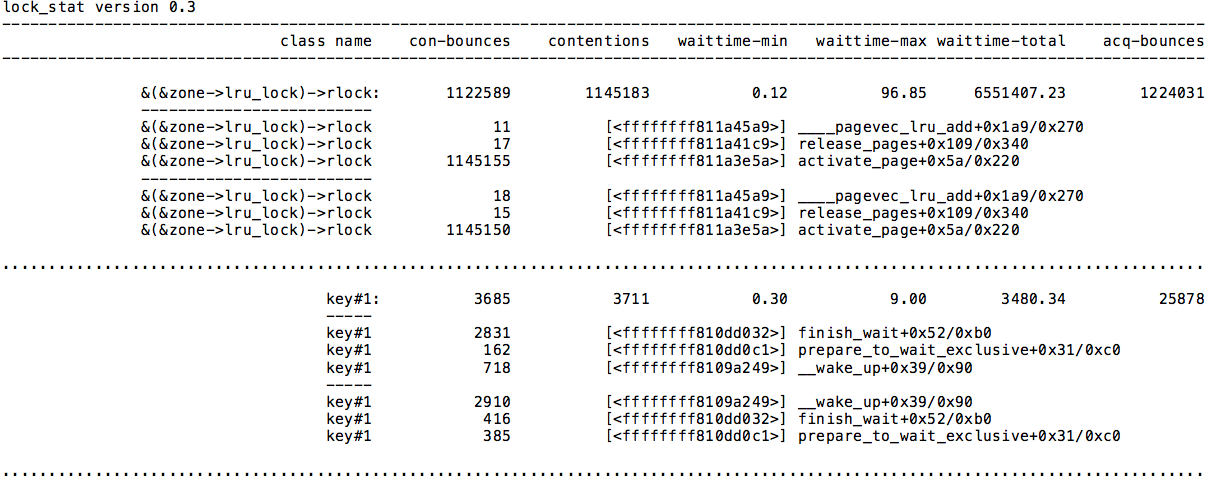
\includegraphics[width=15.3cm]{lock_stat}
\caption{lock\_stat的样例输出}
\label{fig:lock_stat}
\end{figure}

在前面的部分,已经提到lock\_stat记录的是系统中所使用的锁的详细状态。从图\ref{fig:lock_stat}中,我们能够看到:
\begin{enumerate}
\item 系统中不同的锁的状况被长虚线分隔开
\item 属于每一个锁的区域中,第一行是该锁的各项统计数据
\item 最左边是这个锁的名称
\item 第二列表示的是被使用的次数
\item 第三列指的是被使用的函数所在的内存地址
\item 最后一列表示的是这个锁被使用的函数名称以及被调用的代码相对该调用函数的偏移
\end{enumerate}
这些信息对于进行锁的使用分析都是非常必要的。

但是对于性能的分析,我们重点关注的是量化的数字型信息,其他的信息可以不去关注,比如锁的被调用函数的地址以及调用代码的相对偏移等,这些都是可以忽略的信息。

我们在分析lock\_stat这个系统监视器输出的信息的时候,会对每一个锁的调用情况进行分析,结果放到格式化的输出中。

\end{itemize}

\subsubsection{数据格式化}
在对系统监视器的输出内容进行分析之后,我们就可以开始进行数据的格式化了。

在开始格式化之前,我们需要先定义格式化的目标,即需要将系统监视器的内容转换成何种格式。

由于我们进行开发的主要语言是Ruby,而在最新的Ruby中,已经内置了一种简单易懂的数据序列化的保存格式,即YAML。在YAML中,可以保存键值对,可以保存数组和矩阵,更重要的是YAML格式是一种简单易懂的格式,可以被人直接识别,这样可以在很大的程度上降低开发的成本,并且提高开发的效率。因此,在我们的框架中,使用YAML作为所有数据的保存格式。

在YAML中,要表示一组键值对,一般采用下面的格式:
\begin{center}
Key: Value
\end{center}
也就是,在每一组键值对中,键在左边,然后紧跟一个冒号和空格,后面接着和该键对应的值。

在本部分,主要介绍将系统监视器的输出内容格式化为基本的YAML格式,而进一步的处理将会在下一部分中进行介绍。

在YAML中,每一项一般都需要有一个键,为了方便识别和开发,我们采用下面的格式来给每一项进行命名:
\begin{center}
Field.Subfield.Subsubfield.Name
\end{center}
即从左到右不断用该属性所在的域作为后缀,直到到达该键的属性名称。

在对系统键时期的输出结果进行解析的过程中,遇到的时间戳全部都按照原样输出到格式化结果中。

此外,对于每一个不同的系统监视器X,我们都会创建一个名为X.yaml的文件来保存系统监视器X输出内容的格式化结果。

根据上面提到的这些格式化原则, 我们对前面列出的vmstat输出内容的格式化结果为文件vmstat.yaml,而文件vmstat.yaml中的具体内容为:
{\footnotesize
\begin{verbatim}
time: 0.123456
procs.r: 2
procs.b:0
memory.swapd: 0
memory.free 63876
memory.buff: 0
memory.cache: 0
swap.si: 0
swap.so: 0
io.bi: 0
io.bo: 1
system.in: 0
system.cs: 20
cpu.us: 0
cpu.sy: 0
cpu.id: 100
cpu.wa: 0
time: 1.123456
procs.r: 0
...
...
...
\end{verbatim}
}

同理,对于lock\_stat系统监视器的输出内容进行格式化会得到文件lock\_stat.yaml,其中的内容为:
{\footnotesize
\begin{verbatim}
time: 0.123456
&(&zone->lru_lock)->rlock.con-bounces: 112589
&(&zone->lru_lock)->rlock.contentions: 1145183
&(&zone->lru_lock)->rlock.waittime-min: 0.12
&(&zone->lru_lock)->rlock.waittime-max: 96.85
&(&zone->lru_lock)->rlock.waittime-total: 6551407.23
&(&zone->lru_lock)->rlock.acq-bounces: 1224031
&(&zone->lru_lock)->rlock.holdtime-min: 0.10
&(&zone->lru_lock)->rlock.holdtime-max: 5.01
&(&zone->lru_lock)->rlock.holdtime-total: 600953.96
&(&zone->lru_lock)->rlock.contentions.____pagevec_lru_add: 29
&(&zone->lru_lock)->rlock.contentions.release_pages: 32
&(&zone->lru_lock)->rlock.contentions.activate_page: 2290305
...
time: 1.123456
...
...
...
\end{verbatim}
}

\section{测试数据处理}

上一个部分中,已经描述了如何对系统监视器的输出内容进行分析并格式化成YAML格式。对于每一个在测试中执行了监控任务了的系统监视器,在进行系统监视器输出格式化之后都会得到一个以该监视器命名的YAML文件,在这一部分中,我们将会对测试的结果进行进一步的处理和分析。

\subsection{测试数据保存}

为了方便测试数据的管理和保存,在我们的测试框架中,测试的结果都是以文件的形式进行保存的。

在中心任务管理的服务器上,我们创建了一个文件夹专门用于保存所有的测试结果,如
\begin{center}
/test\_result
\end{center}
接下来,我们将根据测试时所使用的测试例程进行分类,根据不同的测试例程分类创建不同的目录,例如在我们的框架中有一个比较简单的测试,是使用Linux系统中自带的dd命令来创建一个比较大的文件,以此来测试I/O的吞吐性能,那么我们将创建一个目录,如
\begin{center}
/test\_result/micro/dd-write
\end{center}

在我们的测试框架中,我们还会在不同的测试环境中进行测试,而在不同的测试环境中进行的测试的测试结果之间显然是没有可比性的,因此,我们还会根据测试环境的不同进行进一步的结果划分,而这种划分将会在文件系统上面得到体现,比如,我们要在只有一个硬盘的机器中分别使用ext4和xfs两种不同的文件系统进行测试,并且在每一次的测试中使用10个dd命令进行测试,那么我们会继续创建下面的目录:
\begin{center}
/test\_result/micro/dd-write/1HDD-ext4-10dd

/test\_result/micro/dd-write/1HDD-xfs-10dd
\end{center}

接下来,我们会根据进行测试的内核版本创建不同的目录,这里的版本指的是在Linux源代码管理的git树中的commit ID,这个commit ID可以帮助我们定位到Linux内核代码树中的每一次的代码修改和更新。假设某一次的commit ID为:
\begin{center}
8bb9660418e05bb1845ac1a2428444d78e322cc7
\end{center}
那么,我们创建下面的文件夹:
\begin{center}
\footnotesize
/test\_result/micro/dd-write/1HDD-ext4-10dd/8bb9660418e05bb1845ac1a2428444d78e322cc7
\end{center}
用来保存该次代码修改之后的内核的性能测试结果。

对于同一个版本的内核,我们很有可能会进行多次的测试,因此,我们会根据测试的次数在对应版本的目录内创建子目录来保存每次测试的测试结果,假设我们进行了3次测试,那么我们创建下面的目录:

\begin{center}
\footnotesize
/test\_result/micro/dd-write/1HDD-ext4-10dd/8bb9660418e05bb1845ac1a2428444d78e322cc7/1

/test\_result/micro/dd-write/1HDD-ext4-10dd/8bb9660418e05bb1845ac1a2428444d78e322cc7/2

/test\_result/micro/dd-write/1HDD-ext4-10dd/8bb9660418e05bb1845ac1a2428444d78e322cc7/3
\end{center}

这样,我们通过这样的目录结构即可对比较复杂的测试结果进行简单清晰地管理,直接使用操作系统自带的文件系统,相对于使用复杂的数据库来说,一方面减少了实现实现上面的复杂度,另一方面减少了对其他组件(如数据库组建)的以来,能够使得整个测试框架更为简洁明了。

\subsection{测试数据的汇总处理}

在完成测试之后,我们能够得到一次的测试结果,但是,一次结果对于性能测试来说是远远不够的,要对内核的性能进行比较完整准确的分析,我们需要大量的测试结果作为参考。为了能够管理好测试的历史记录,我们会在每次处理测试结果的时候将结果进行汇总。

在开始处理测试数据的时候,我们首先得到的是由系统监视器产生的YAML文件和描述该次测试任务的YAML描述文件。

对于所有由系统监视器输出结果格式化得到的YAML文件,我们将全部汇总到该次测试的结果目录下的stats.yaml文件中,在每一个键的名字之前添加该监视器的名称作为限定,对应的值则是一个数组,是由不同时间段产生的数据汇总而成的。

假设某个vmstat.yaml的内容如下:
\begin{verbatim}
time: 0.123456
procs.r: 2
...
time: 1.123456
procs.r: 1
...
time: 2.123456
procs.r: 3
...
\end{verbatim}
那么对应的内容在stats.yaml的表示为:
\begin{verbatim}
...
vmstat.procs.r: [ 2, 1, 3 ]
...
\end{verbatim}
每一次生成stats.yaml文件之后,我们还会对应地生成平均值和标准方差的数据文件avg.yaml和stddev.yaml。

另外,对于每一个进行测试的内核,在对应commit ID的文件夹下都会有一个名为matrix,yaml文件用来汇总所有stats.yaml中的数据。

在后面的性能回退算法中,我们还会介绍进一步的数据处理步骤。
\subsection{测试数据的可视化比较}
在我们的测试框架中,我们除了能够进行自动化的性能回退判断分析,还可以提供方便人工分析的图表比较功能。

在实现上,我们会通过读取stats.yaml和avg.yaml来进行分析和比较,在画图方面,我们将使用GnuPlot来进行画图。通过stats.yaml和avg.yaml,我们可以进行同一个内核多次测试的比较,也可以进行不同内核的测试平均值的比较,还能比较不同的测试参数下的测试结果。



使用GnuPlot进行画图。
